\section{更新方法(初次阅读使用可跳过)}
\label{how_to_update}

\textbf{\color{red}对 v1.3.x 或更早版本的用户,需要注意:\lstinline{lua} 目录已经更名为 \lstinline{Executor}。}

在迁移到 v1.5.x 版本时,\textbf{\color{red}强烈建议}先阅读第三章(篇幅已经大幅缩短)以了解在 v1.5.x 中发生了哪些新变化。

下载新版集成工具压缩包并解压后(注意需解除锁定),在 Powershell 中运行 \lstinline{install.ps1}(运行前需注意是否已经按照第一章所属步骤修改 Powershell 执行策略),运行后会在当前目录下生成一个名为 \lstinline{Executor.lua} 的文件。

点击此链接 \href{https://www.macrohard.fun/CSOL-Utilities/ConfigPanel}{CSOL 集成工具配置面板} 打开配置面板。

在网页最下方点击“导入”,将您的旧版集成工具使用的 \lstinline{Setting.lua} 文件导入。

\begin{figure}[H]
    \Centering
    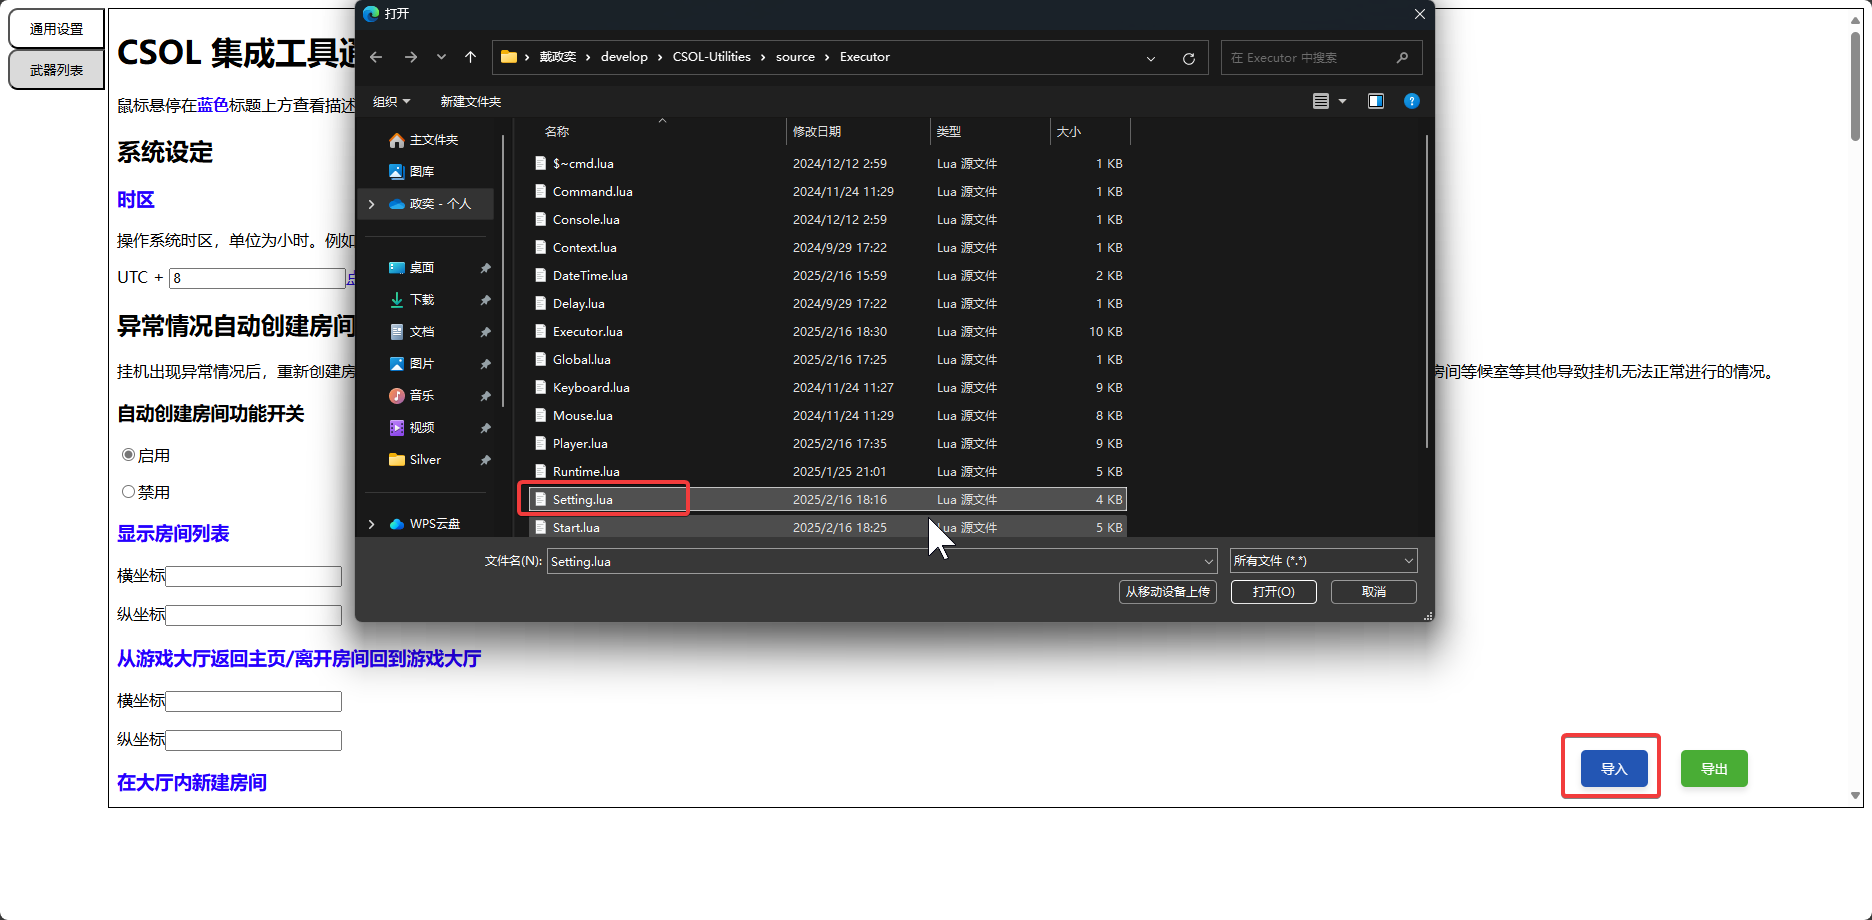
\includegraphics[width=\textwidth]{assets/import_setting}
    \caption{导入旧版集成工具使用的 \lstinline{Setting.lua}}
\end{figure}

\textbf{\color{red}若您有修改配置文件中某些坐标的需求,则先使用旧版工具定位这些坐标,并在网页中相应位置进行修改。}

然后,点击最下方的“导出”,若存在尚未配置的字段,则网页会弹出提示,根据提示填补缺失的字段即可。

\begin{figure}[H]
    \Centering
    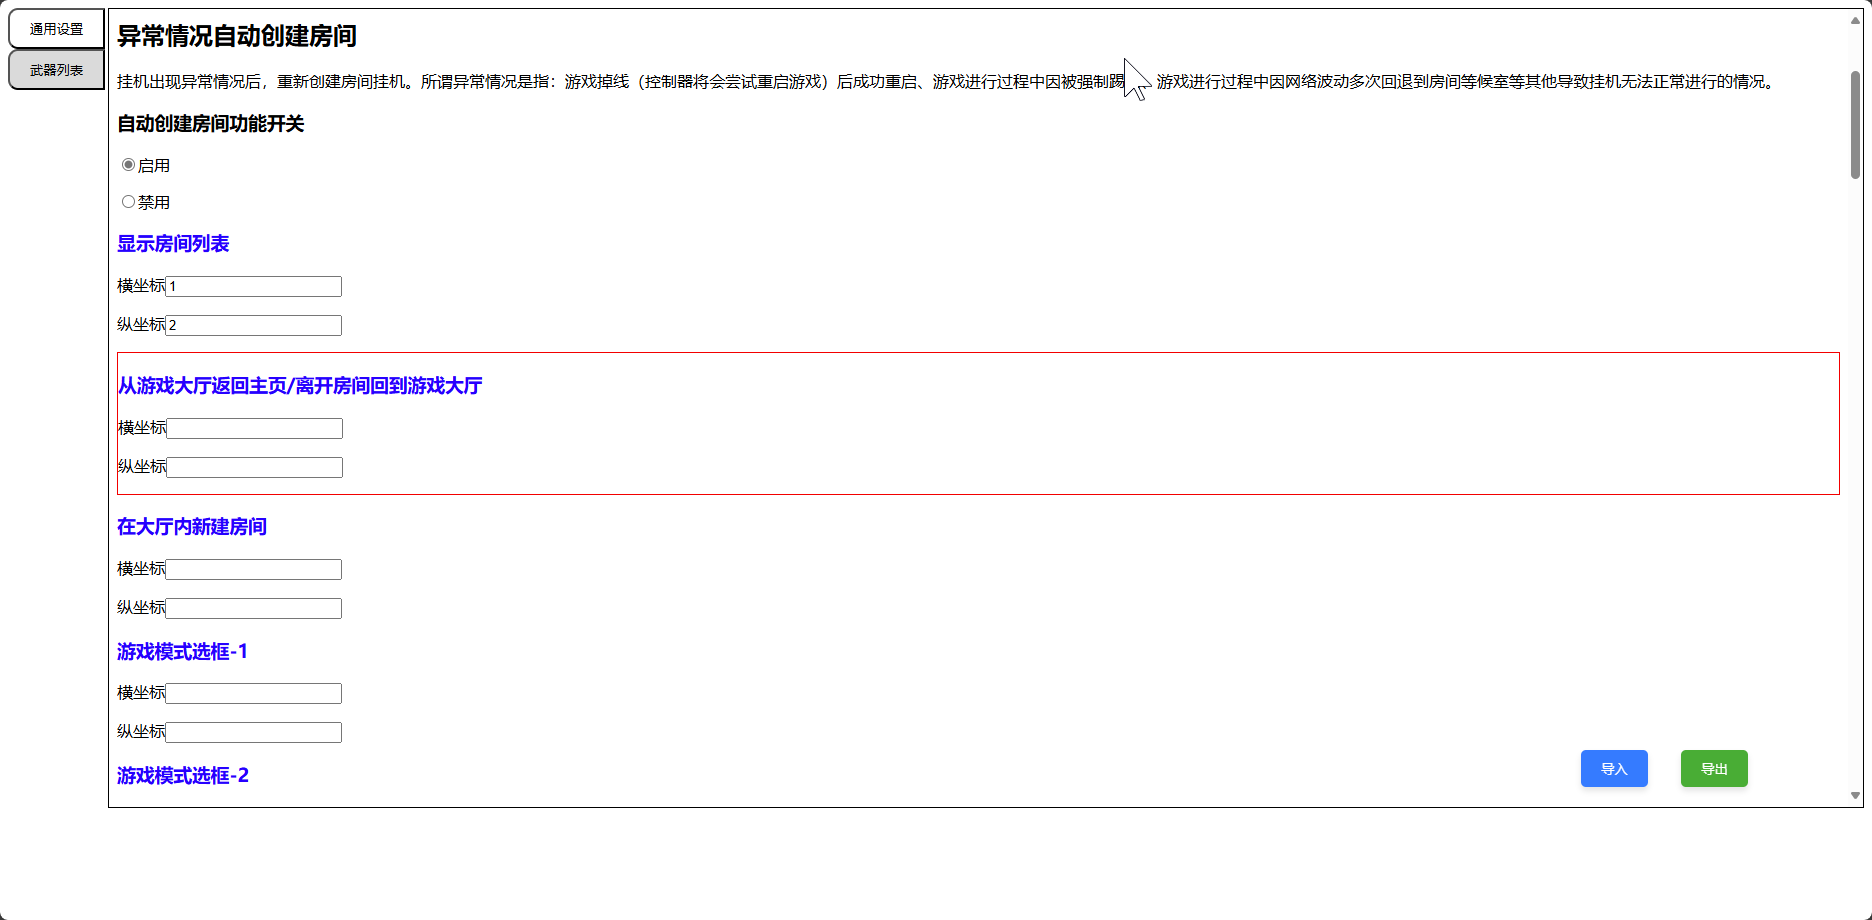
\includegraphics[width=\textwidth]{assets/export_error}
    \caption{根据网页提示的信息填补缺失字段}
\end{figure}

上述操作完成后,导出 \lstinline{Setting.lua} 到\textbf{\color{red}新版集成工具}的 \lstinline{Executor} 目录下,\textbf{\color{red}覆盖}原有的 \lstinline{Setting.lua} 文件。然后,\textbf{\color{red}将新工具目录下的 \lstinline{Executor.lua} 导入罗技软件并保存运行。}

\begin{figure}[H]
    \Centering
    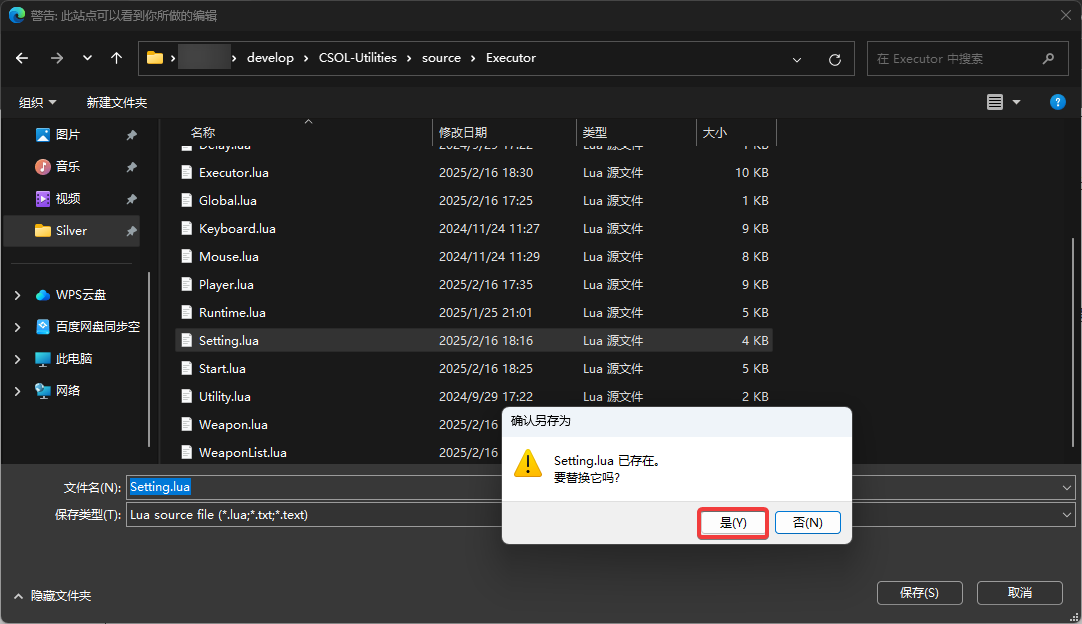
\includegraphics[width=\textwidth]{assets/override_setting}
    \caption{导出 \lstinline{Setting.lua}}
\end{figure}

对于武器列表,采用同样的方法,将旧版集成工具使用的 \lstinline{WeaponList.lua} 文件导入配置面板,视自身需要进行修改,然后导出。导出时,覆盖原有的 \lstinline{WeaponList.lua} 文件。

在罗技软件中导入并运行新的 \lstinline{Executor.lua} 使您的配置生效。

最后,关闭旧版的控制器和 GamingTool(任务栏中的小图标)。并运行新版 \lstinline{Controller.ps1} 和 \lstinline{GamingTool.exe} 即可正常使用。

\begin{figure}[H]
    \Centering
    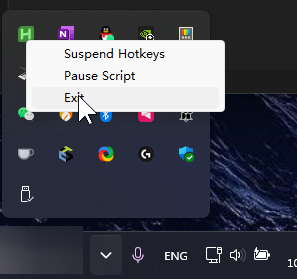
\includegraphics[width=\textwidth]{assets/intro/exit_gamingtool}
    \caption{退出 GamingTool}
\end{figure}